\documentclass[10pt,hyperref={pdfpagelabels=false},xcolor=table]{beamer}
\usepackage{multicol}

% Contact information: 
%   Jorge M. Cruz-Duarte (jorge.cruz@tec.mx)
%   Nov. 29, 2019

\usepackage{lmodern, ragged2e, CJKutf8, booktabs, subfig,adjustbox, graphicx, amsmath, amssymb, amsthm, amsfonts, mathtools, multirow,wrapfig,lipsum,tikz, tikz-cd,tikz-3dplot,pgfplots,minted}
\usepackage[style=phys]{biblatex}
\usepackage[lined,boxed,vlined,ruled,linesnumbered]{algorithm2e}
\SetKw{Continue}{continue}
\SetKw{Or}{or}
\SetKw{Until}{until}
\addbibresource{bibliography.bib}
\renewcommand{\footnotesize}{\tiny}
\newcommand{\norm}[1]{\left\lVert#1\right\rVert}
\makeatletter
\@newctr{footnote}[page]
\makeatother

\usetheme{CambridgeUS}
\renewcommand{\raggedright}{\leftskip=0pt \rightskip=0pt plus 0cm}

\definecolor{UQPurple}{RGB}{0, 32, 159}
% This is the trademark pruple that UQ uses
\definecolor{UQPurple}{RGB}{81,36,122}
\newcommand{\hl}[1]{{\textcolor{UQPurple}{#1}}}

% Theme setup
\titlegraphic{\includegraphics[scale=0.05]{img/UQ_color_logo.png}}

% \makeatletter
\setbeamertemplate{headline}{%
  \leavevmode%
  \hbox{%
    \begin{beamercolorbox}[wd=\paperwidth,ht=2.5ex,dp=1.125ex]{palette quaternary}%
      \insertsectionnavigationhorizontal{\paperwidth}{}{\hskip0pt plus1filll}
    \end{beamercolorbox}%
  }
}
\setbeamertemplate{footline}{\hspace*{2ex} \insertshortauthor \hfill \textcolor{UQPurple}{\insertshorttitle} \hfill \textbf{\insertframenumber{}} / \inserttotalframenumber \hspace*{2ex}}

\setbeamercolor{item projected}{bg=UQPurple}
\setbeamertemplate{enumerate items}[default]
\setbeamercolor*{enumerate item}{fg=UQPurple}

\setbeamertemplate{navigation symbols}{}
% \setbeamertemplate{footline}[\insertshorttitle frame number]
\setbeamertemplate{bibliography item}[text]
\setbeamertemplate{theorems}[numbered]

\setbeamerfont{title}{series = \bfseries, parent = structure}
\setbeamerfont{frametitle}{series = \bfseries, parent = structure}
\setbeamerfont{headline}{series = \bfseries, size = \tiny, parent = structure}

\setbeamercolor{title}{fg = white, bg = UQPurple}
\setbeamercolor{frametitle}{fg = white, bg = UQPurple}
\setbeamercolor{structure}{fg = UQPurple}
\setbeamercolor{section in head/foot}{fg = black, bg = UQPurple!40}
\setbeamercolor{subsection in head/foot}{fg = black, bg = UQPurple!20}

\setbeamercolor{block title}{use=structure,fg=white,bg=structure.fg!75!black}
\setbeamercolor{block body}{parent=normal text,use=block title,bg=UQPurple!20} %block title.bg!10!bg}
\makeatletter
\def\th@mystyle{%
  \normalfont % body font
  \setbeamercolor{block title example}{bg=orange,fg=white}
  \setbeamercolor{block body example}{bg=orange!20,fg=black}
  \def\inserttheoremblockenv{exampleblock}
}
\makeatother
\theoremstyle{mystyle}
\newtheorem*{remark}{Remark}

\usepackage{tikz,color,xcolor,amsmath,amsfonts,stmaryrd,amssymb,bm}
\usepackage{url}

%Just having a look at what it looks like without it
\setbeamertemplate{background}{\tikz[overlay,remember picture]\node[opacity=0.07]at (current page.center){\includegraphics[width=6cm]{img/UQ_purple_logo.png}};}


\newcommand{\maketitleandtoc}{%
  {%
      \setbeamertemplate{headline}{}%
      \setbeamertemplate{footline}{}%
      \begin{frame}[noframenumbering]%
        \titlepage%
      \end{frame}%
      \begin{frame}[noframenumbering]%
        \frametitle{Outline}%
        \tableofcontents%
      \end{frame}%
    }}

\newcommand{\noheadfoot}[1]{%
  {%
      \setbeamertemplate{headline}{}%
      \setbeamertemplate{footline}{}%
      {#1}
    }
}

\title{Optimizing Gaussian Processes}  
\author[Michael Ciccotosto-Camp]{{\bf Honours Research Project}} 
%\institute{}
\date{
Michael Ciccotosto-Camp - 44302913 \\
}

\begin{document}

\maketitle

\section{Problem Significance}

\begin{frame}
    \frametitle{Problem Setting and Motivation}
    \begin{itemize}
        \item This project focuses on the problem of time series prediction.
        \item Given a data set of $n$ observations $\mathcal{D} = \left\{ \left( x_i , y_i \right) \right\}_{i=1}^{n}$, where each input $x_i \in \mathbb{R}_{>0}$ is a time value and $y_i \in \mathbb{R}$ is a output or experimental observation that acts a function of time, the goal of time series prediction is to try and best predict a value $y_{\star}$ at time $x_{\star}$.
        \item The idea of studying time series prediction came from a research group from the Gatton campus, lead by Andries Potgieter, analysing crop growth from previous seasons to forecast when certain phenological stages will take place in the current harvest.
    \end{itemize}
    \begin{figure}
        \centering
        \includegraphics[scale=0.18]{img/yan_wheat_GPR_plot.png}
    \end{figure}
\end{frame}

\begin{frame}
    \begin{figure}
        \centering
        \frametitle{Infrared Spectroscopy and Mass Spectrum Data}
        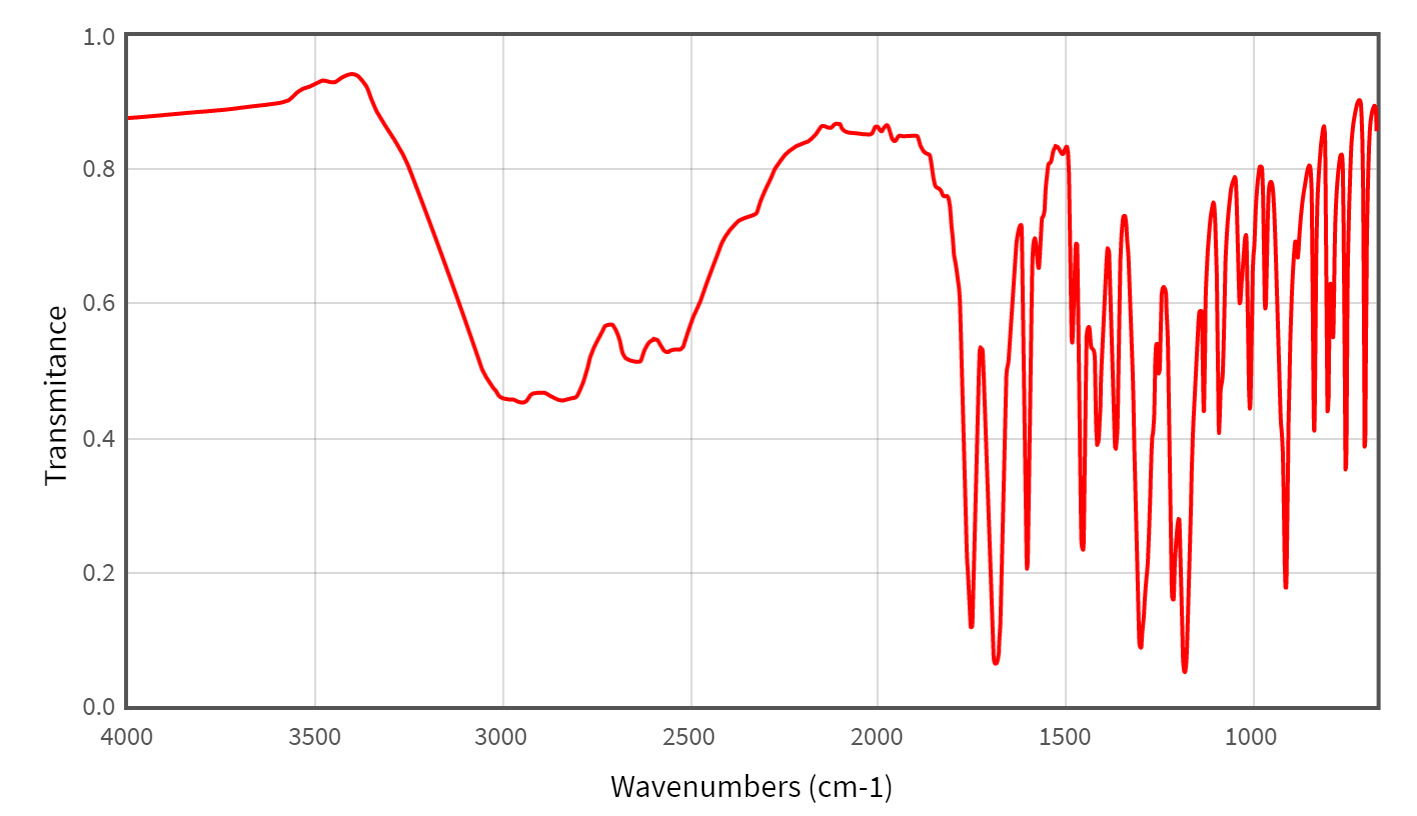
\includegraphics[scale=0.35]{aspirin_IR}
        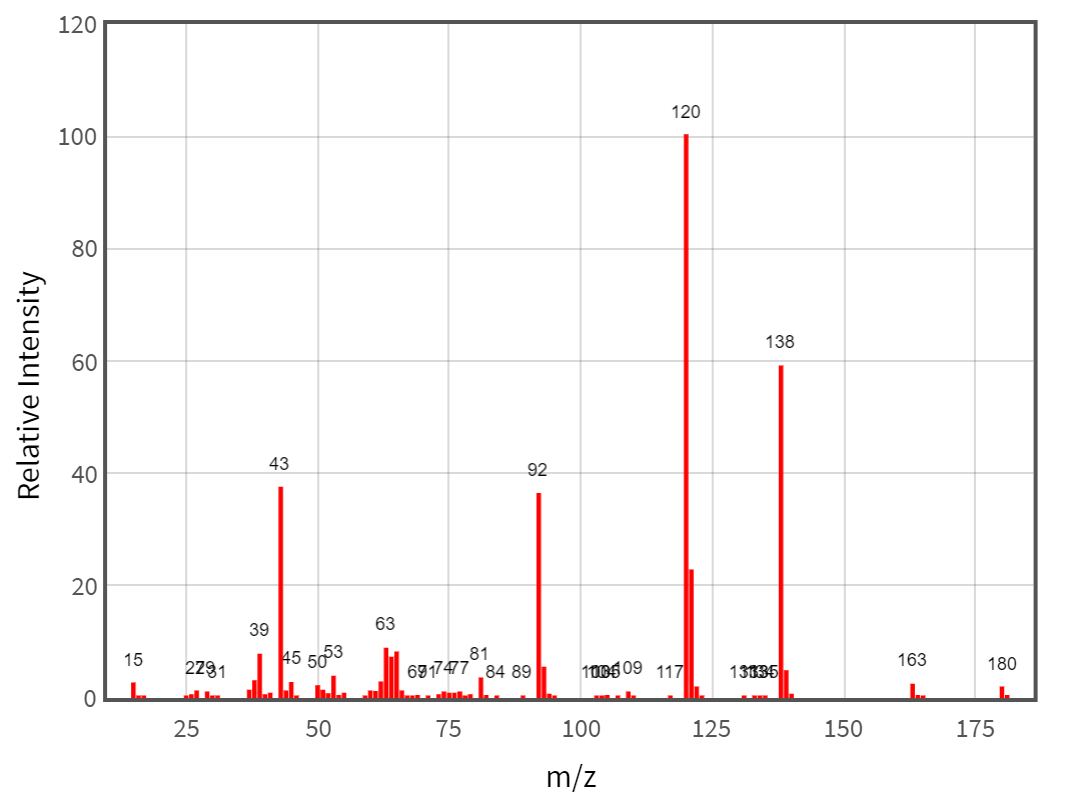
\includegraphics[scale=0.35]{MS _data_aspirin}
    \end{figure}
    \begin{itemize}
        \item \textbf{Project Goal:} Develop a deep learning model to accurately predict functional groups based off Infrared (IR) and Mass Spectrometry (MS) data \footfullcite{NIST}. Main focus will be on Multi-layer Perceptrons (MLPs).
    \end{itemize}

\end{frame}




\end{document}

